  \subsection{The decision procedure}  
  The decision procedure is defined as a set of derivation rules. The procedure starts with an initial configuration keeps applying the derivation rules according to the strategy. During this repeated application of rules a derivation tree is produced.  When any rule is selected for application, it may cause the tree to branch at this configuration. These  rules are usually called spiting rules. A configuration may be \texttt{unsat}. If the procedure reaches a configuration which is \texttt{unsat}, it will backtrack and choose another branch for rule application. If there is no other branch in case of \texttt{unsat}, we call the branch is closed. Another possibility is that, the procedure reaches a configuration, where no more rule application is possible. Such a configuration is a $staturated$ one. A derivation tree is called $closed$ if all of its branches are closed. If the procedure ends up with a closed derivation tree, it concludes that the set of constraints are unsatisfiable or declares \texttt{unsat}. On the other hand,  If the procedure ends up with a saturated configuration, it concludes that the set of constraints are satisfiable or declares \texttt{unsat}. Whenever any new string constraint is derived from any rule application, the procedure restart. 
      
  At the start of the procedure, each term in the set of constraints must be in their normalized form according to the reduction rules listed below.   

					  \begin{align*}
					  \texttt{con}(\mathbf{s},  \texttt{con}(\mathbf{t}), \mathbf{u}) &\rightarrow   \texttt{con}(\mathbf{s},\mathbf{t}, \mathbf{u})\\
					  \texttt{con}(\mathbf{s}, \epsilon, \mathbf{u}) &\rightarrow \texttt{con}(\mathbf{s}, \mathbf{u})\\
					  \texttt{con}(s) &\rightarrow s\\
					  \texttt{con}() &\rightarrow \epsilon\\
					  \texttt{con}(\mathbf{s}, c_1 \cdots c_i, c_{i+1} \cdots c_n, \mathbf{u}) &\rightarrow \texttt{con}(\mathbf{s}, c_1 \cdots c_n, \mathbf{u})\\
					  \texttt{len}( \texttt{con}(s_1,\cdots,s_n)) &\rightarrow \texttt{len}(s_1) + \cdots + \texttt{len}(s_n)\\
					  \texttt{len}(c_1,\cdots,c_n) &\rightarrow n
					  \end{align*}					 
  Here is few examples of terms and their normal forms, 
  $\texttt{con}("ab", \texttt{con}("c", l)) \rightarrow \texttt{con}("abc",l) $, $\texttt{len}("abc") \rightarrow 3$,\\ $\texttt{len}(\texttt{con}("abc", "def"))\rightarrow 6$. 
  
  
  The procedure starts applying rules on the initial configuration according to the following steps:
  \begin{enumerate}   
    \item $Check\ conflicts:$ The idea is to drive conflict as early as possible. Apply \texttt{S-Conflict} or \texttt{A-Conflict} to check if the configuration is unsatisfiable due to the current string or arithmetic constraints. 
\begin{align*}
 \texttt{A-Conflict} &\frac{ A \models_{LIA} \perp }{ \textnormal{unsat}}\\  
 \texttt{S-Conflict} &\frac{ s\approx t \in S \ \ s \not\approx t \in S}{\textnormal{unsat}}
\end{align*}
    
         Examples of the  application are:  $S:\{ \cdots, x \approx \epsilon,x\not\approx \epsilon, \cdots\} \rightarrow{\texttt{unsat}}$, $S:\{ \cdots, x \approx y,x\not\approx y, \cdots\} \rightarrow{\texttt{unsat}}$, $A:\{ \texttt{len}(x) \approx \texttt{len}(y), \texttt{len}(x) \not\approx \texttt{len}(y) \}\rightarrow{\texttt{unsat}}$      
      
    \item $Propagate:$ Introduce new constraints induced by constraints in other theories (e.g. $\mathcal{T}_{LIA}$ and $\mathcal{T}_{SL} $). 
        \begin{align*}
     \texttt{A-Prop} &\frac{ S \models  \texttt{len} \ x \approx \texttt{len} \ y}{ A := A, \texttt{len} \ x \approx \texttt{len} \ y}\\
      \texttt{S-Prop} &\frac{ A \models_{LIA}  \texttt{len} \ x \approx \texttt{len} \ y}{ S := S, \texttt{len} \ x \approx \texttt{len} \ y}
          \end{align*}
        
     Examples of the application are: $S \models (\texttt{len} \ x \approx \texttt{len} \ y) \rightarrow A:=A,{\texttt{len} \ x \approx \texttt{len} \ y}$, $S \models (\texttt{len} \ x \approx \texttt{len} \ "abc") \rightarrow A:=A,{\texttt{len} \ x = 3 }$

    
    
    
    
    
    \item $Split\ by\ Length:$ Introduce new constraint to the arithmetic constraints for equalities in string constraints. Introduce branching for free variables in string constraints with \texttt{Len-Split}.     		
    			\begin{align*} 
    			\texttt{Len} &\frac{ x \approx t \in \mathcal{C}(S) \ x \in \mathcal{V}(S)}{ A := A, \texttt{len} \ x \approx (\texttt{len} \ t) \downarrow}\\
    			\texttt{Len-Split} &\frac{ x \in \mathcal{V}(S \cup A) \ x: Str}{ S := S, x \approx \epsilon \parallel  A:= A, \texttt{len} \ x > 0}
    			\end{align*}    		
   Examples of the application are: $S \models (x \approx y) \rightarrow A:=A,{\texttt{len} \ x \approx \texttt{len} \ y}$, $S \models (x \approx "abc") \rightarrow A:=A,{\texttt{len} \ x = 3 }$     
    
    
    \item $Normalize:$ Compute the normalized form for each term. As in the previous steps we may have added new constraints to the set of constraints we started with. So these terms should be normalized as per the normalization reduction rules. Apply \texttt{S-Cycle} to shrink the concatenation terms. Then apply the normalization rules   \texttt{F-Form1}, \texttt{F-Form2}, \texttt{N-Form1} and \texttt{F-Form2} to the completion. The idea is to produce a total map of normal forms. If still there exists any term, which is not in its normalized form first apply splitting and then finally unify.
    		
    			\begin{align*}
    			\texttt{F-Unify} &\frac
    			{ F \ s = ( w,u,u_1) \ \ F \ t = (w, u,v_1) \  s\approx t \in \mathcal{C}(S) \ S \models \textnormal{len} \ u \approx \textnormal{len} \ v }
    			{ S:= S, u \approx v}
    			\end{align*}
    		
    		Examples of the application is : $\texttt{con}(x, m) \approx \texttt{con}(y, n) , \texttt{len}(x) \approx \texttt{len}(y)  \rightarrow S:=S,{ x \approx  y}$.
    
    \item $Partition:$ 
    Each equivalence class should be in their corresponding group (bucket). The target is to distribute each equivalence class to a bucket. This classification is done on the expected length of the value. First apply \texttt{D-Base} and \texttt{D-Add} to completion. If the partition is not compete, splitting is required for the free variables. That is , at this point of rule application, there exits an equivalence class which is not contained in any bucket. At this step rules like \texttt{S-Split}, \texttt{D-Split}, \texttt{L-Split} are applied according to different cases. 
     		\begin{align*}
    		\texttt{S-Split} &\frac
    		{ x, y \in \mathcal{V}(S) \ \ x \approx y, x \not\approx y \in \mathcal{C}(S) }
    		{ S := S, x \approx y \parallel S:= S, x \not\approx y}\\
    		\texttt{L-Split} &\frac
    		{ x, y \in \mathcal{V}(S) \ \ x,y: \textnormal{Str}  \ \  S \not\models \texttt{len} \ x \not\approx \textnormal{len} \ y}
    		{ S:= S, \textnormal{len} \ x \approx \texttt{len} \ y \parallel S:=S, \textnormal{len} \ x \not\approx \texttt{len} \ y}
    		\end{align*}
    Otherwise the procedure have reached a saturated configuration.    
    \item $Check\ cardinality:$ This is the last step of the procedure. The procedure has reached a saturated configuration. Now for each bucket B the procedure introduce new arithmetic constraints corresponding to the minimal length of terms in $B$ based on the number of equivalence classes in $B$ and the cardinality $| 
    \mathcal{A}|$ of the alphabet. 
  \end{enumerate}
  
   \begin{figure}[htb]
   	\centering
   	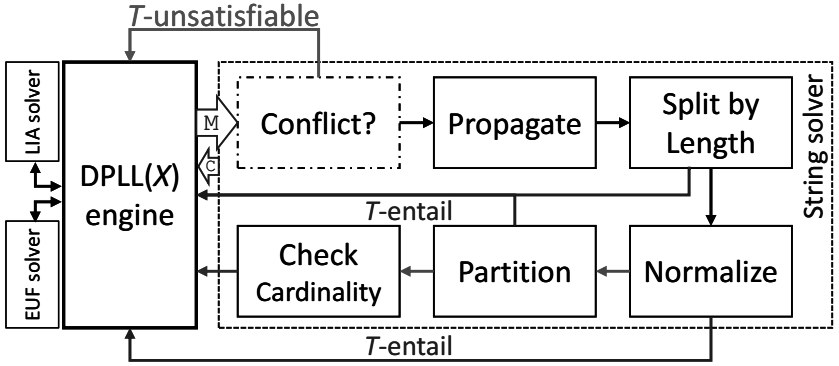
\includegraphics[width=0.7\linewidth]{pictures/proof_procedure.png}
   	\caption{Abstracted core proof procedure for string. The figure is sourced from \cite{main_phd}.}
   	\label{fig:proof_procedure}
   \end{figure}
  Figure \ref{fig:proof_procedure} shows the overall application strategy. The full list of derivation rules can be found in Figures from \ref{rules_1} to \ref{rules_5}. The four rules $\texttt{A-Prop},\texttt{S-Prop},\texttt{Len}$ and $\texttt{Len-Splite}$  in Figure \ref{rules_1} describe the interaction between arithmetic solver and string solver. This is achieved via the propagation of entailed constraints on the shared terms. This technique of cooperation between different theory solvers is well know as Nelson-Oppen method \cite{nelson_oppen}. The rule \texttt{S- Split}  tries to guess whether two strings are equal or not, while \texttt{L-Split} tries to guess whether two string variables have the same length.  Application of split rules causes the branching of the derivation tree. Whenever any new constraints are introduced to the set $S$, the procedure restart. Finally, when the procedure reached the saturated configuration, the rule \texttt{Card} makes sure that each bucket has been assigned big enough length. Detail about the individual rule can be found in \cite{main_phd} and in \cite{main-paper}.
 
 \begin{figure}
\scriptsize
\begin{minipage}{1.0\textwidth}
\begin{gather*}\label{eA1}
 \texttt{A-Prop} \frac{ S \models  \texttt{len} \ x \approx \texttt{len} \ y}{ A := A, \texttt{len} \ x \approx \texttt{len} \ y}\\
  \texttt{S-Prop} \frac{ A \models_{LIA}  \texttt{len} \ x \approx \texttt{len} \ y}{ S := S, \texttt{len} \ x \approx \texttt{len} \ y}\\
 \texttt{Len} \frac{ x \approx t \in \mathcal{C}(S) \ x \in \mathcal{V}(S)}{ A := A, \texttt{len} \ x \approx (\texttt{len} \ t) \downarrow}\\
 \texttt{Len-Split} \frac{ x \in \mathcal{V}(S \cup A) \ x: Str}{ S := S, x \approx \epsilon \parallel  A:= A, \texttt{len} \ x > 0}\\
 \texttt{A-Conflict} \frac{ A \models_{LIA} \perp }{ \texttt{unsat}}\\
 \texttt{R-Star} \frac{ s \ in \ star( set \ t) \in R \ s  \not\approx \epsilon \in \mathcal{C}(S)}{ S:= S, s \approx \textnormal{con}(t,z) \textnormal{R}:= \textnormal{R}, z \ in \ star \ (set \ t)}
\end{gather*}
\end{minipage}
\caption{ The rules for theory combination\cite{main-paper}. \texttt{R-Start} is handle cases with regular expression. }
\label{rules_1}
\end{figure}
 \begin{figure}
\begin{minipage}{1.0\textwidth}
\scriptsize
\begin{gather*}\label{eA1}
 \texttt{S-Cycle} \frac
 { t = \texttt{con}(t_1, \cdots, t_i, \cdots, t_n) \ t \in \mathcal{T}(S) \setminus C \ t_k \approx \epsilon \in \mathcal{C}(S) \ \textnormal{for all} \ k \in \{1,\cdots,n\} \setminus \{ i \} }
 { S := S, t \approx t_i \ C:=C (C, t) \setminus \{t_i\}   }\\
  \texttt{Reset} \frac{ }
  { \textnormal{F} := \phi, \textnormal{N} := \phi, \textnormal{B} := \phi}\\
   \texttt{S-Split} \frac
   { x, y \in \mathcal{V}(S) \ \ x \approx y, x \not\approx y \in \mathcal{C}(S) }
   { S := S, x \approx y \parallel S:= S, x \not\approx y}\\
      \texttt{S-Conflict} \frac
      { x \approx t \in \mathcal{C}(S) \ \ s \not\approx t \in \mathcal{C}(S)}
      { \textnormal{unsat}}\\
      \texttt{L-Split} \frac
       { x, y \in \mathcal{V}(S) \ \ x,y: \textnormal{Str}  \ \  S \not\models \texttt{len} \ x \not\approx \texttt{len} \ y}
       { S:= S, \texttt{len} \ x \approx \texttt{len} \ y \parallel S:=S, \texttt{len} \ x \not\approx \texttt{len} \ y}
\end{gather*}
\end{minipage}
\caption{Basic string derivation rules \cite{main-paper}.}
\label{rules_2}
\end{figure}

 \begin{figure}
\begin{minipage}{1.0\textwidth}
\scriptsize
\begin{gather*}\label{eA1}
 \bold{F-Form1} \frac
 { t = \textnormal{con}(t_1, \cdots,t_n) \ t \in \mathcal{T}(S) \setminus ( \mathcal{D}(F) \cup C)  \ \  N[t_1] = s_1 \cdots N[t_n] = s_n }
 { \textnormal{F} := \textnormal{F}, t \mapsto ( s_1, \cdots, s_n) \downarrow}\\
 \bold{F-Form2} \frac
 { l \in \mathcal{T}(S) \setminus \mathcal{D}(F)}
 { \textnormal{F} := \textnormal{F}, t \mapsto ( l)} \\
  \bold{N-Form1} \frac
  { [x] \not\in \mathcal{D}(N) \ \ s \in [x] \setminus ( C \cup \mathcal{V}(S)) \ \ F t= F s \textnormal{for all} \ t \in [x] \setminus ( C \cup \mathcal{V}(S)) }
  { \textnormal{N}:= \textnormal{N}, [x] \mapsto F s}\\
  \bold{N-Form2} \frac
  { [x] \not\in \mathcal{D}(N) \ \ [x] \subseteq  C \cup \mathcal{V}(S)} 
  { \textnormal{N}:= \textnormal{N}, [x] \mapsto (x)}
\end{gather*}
\null
\par\xdef\tpd{\the\prevdepth}
\end{minipage}
\caption{Normalization derivation rules. The letter \(l\) denotes a string constant.The rules are taken from \cite{main-paper} and they are in their original form.}
\label{rules_3}
\end{figure}
 \begin{figure}
\begin{minipage}{1.0\textwidth}
\scriptsize
\begin{gather*}\label{eA1}
 \texttt{F-Unify} \frac
 { F \ s = ( w,u,u_1) \ \ F \ t = (w, u,v_1)  s\approx t \in \mathcal{C}(S) \ S \models \texttt{len} \ u \approx \texttt{len} \ v }
 { S:= S, u \approx v}\\
  \texttt{F-Split} \frac
  {\parbox{3.2in}{$  F \ s = ( w,u,u_1) \ \ F \ t = (w, u,v_1)  s\approx t \in \mathcal{C}(S) \ S \models \texttt{len} u \approx \texttt{len} \ v  $ \\
       \hspace*{2.0cm}$ u \not\in \mathcal{V}(v_1) \ v \not\in \mathcal{V}(u_1)$}}
  { S:= S, u \approx con(v, z) \parallel  S:= S, v \approx con(u, z) }\\
  \texttt{F-Loop} \frac
  { F \ s = ( w,x,u_1) \ \ F \ t = (w, u,v_1, x, v_2)  \ s\approx t \in \mathcal{C}(S) \ x \not\in \mathcal{V}((v,v1))}
  { \parbox{3.6in}{$ S:= S, x \approx con(z_2, z),\ con(v,v1) \approx con(z_2,z_1),\ con(u_1) \approx con( z_1, z_2,v_2)$ \\
   \hspace*{2.0cm}$  R:=R, z \ in \ star(set \ con(z_1, z_2)) \ \ C:=C, t $}}
\end{gather*}
\end{minipage}
\caption{The rules for equality reduction \cite{main-paper}. The rule \texttt{F-Loop} is used to detect looping problem.}
\label{rules_4}
\end{figure}
 \begin{figure}
\begin{minipage}{1.0\textwidth}
\scriptsize
\begin{gather*}\label{eA1}
 \texttt{D-Base} \frac
 { s \in \mathcal{T}(S) \ \ s: \textnormal{Str}  \ \  S \models \textnormal{len} \ s \approx \textnormal{len}_B \textnormal{ for no }  B \in B }
 { B:= B, \{ [s]\}}\\
  \texttt{Card} \frac
  {B \in B \ \ |B| > 1}
  { A:= A, \textnormal{len}_B >  \lfloor  log_{| \mathcal{A}|}  \ ( |B| -1) \rfloor }\\
  \texttt{D-Add} \frac
  { \parbox{3.3in}{\hspace*{0.5cm} $s \in \mathcal{T}(S) \ \ s: \textnormal{Str} \ \ B = \textnormal{B'}, B \   S \models \textnormal{len} \ s \approx \textnormal{len}_B  [s]  \not\in B 
  		$ \\
  		\hspace*{0.8cm}$  		\textnormal{ for all }  e \in B \textnormal{ there are } w, u,u_1, v,v_1 \textnormal{ such that} 
  		 $ \\
  		 \hspace*{0.0cm}$ (N [s] = (w, u,u_1), N e = (w, v,v1), \ S \models \textnormal{len} \ u \approx \textnormal{len} v, u \not\approx v \in \mathcal{C}(S))$}}
  { B:= B', ( B \cup \{ [s]\})}\\
  \texttt{D-Split} \frac
  { \parbox{4.0in}{\hspace*{1.5cm} $s \in \mathcal{T}(S) \ \ s: \textnormal{Str} \ \ B = \textnormal{B'}, B \   S \models \textnormal{len} \ s \approx \textnormal{len}_B  [s]  \not\in B \ e \in B   		 
  		$ \\
  		\hspace*{2cm}$ (N [s] = (w, u,u_1), N e = (w, v,v1), \ S \models \textnormal{len} \ u \not\approx \textnormal{len}\ v $}}
  {  S:=S, u \approx con(z_1, z_2), len \ z_1 \approx len \ v  \parallel  S:=S, v \approx con(z_1, z_2), len \ z_1 \approx len \ u}
  \end{gather*}
 \end{minipage}
\caption{The rules for dis-equality reduction\cite{main-paper}.}
\label{rules_5}
\end{figure}